\documentclass{article}
\usepackage{problem-set}

\begin{document}

\tableofcontents

\CHAPTER{10}

\subsection*{Problem 10.1}
\addcontentsline{toc}{subsection}{Problem 10.1}
Assuming the validity of Raoult's law, do the following calculations
for the benzene(1)/toluene(2) system:
\begin{enumerate}[label=(\alph*)]
  \item Given $x_{1} = 0.33$ and $T=100~\unit{\degreeCelsius}$, find
    $y_{1}$ and $P$.
  \item Given $y_{1} = 0.33$ and $T=100~\unit{\degreeCelsius}$, find
    $x_{1}$ and $P$.
  \item Given $x_{1} = 0.33$ and $P=120~\unit{\kilo\pascal}$, find
    $y_{1}$ and $T$.
  \item Given $y_{1} = 0.33$ and $P=120~\unit{\kilo\pascal}$, find
    $x_{1}$ and $T$.
  \item Given $T=105~\unit{\degreeCelsius}$ and
    $P=120~\unit{\kilo\pascal}$ find $x_{1}$ and $y_{1}$.
  \item For part (e), if the \textit{overall} mole fraction of
    benzene is $z_{1}=0.33$, what molar fraction of the two-phase
    system is vapor?
  \item Why is Raoult's law likely to be an excellent VLE model for
    this system at the stated (or computed) conditions?
\end{enumerate}
\begin{solution}
  \begin{align*}
    A_{1} = 13.7819 & \qquad A_{2} = 13.9320 \\
    B_{1} = 2726.81 & \qquad B_{2} = 3056.96 \\
    C_{1} = 217.572 & \qquad C_{2} = 217.625
  \end{align*}
  \begin{enumerate}[label=(\alph*)]
    \item $x_{1}=0.33$ and $T=100~\unit{\degreeCelsius}$, find $P$ and $y_{1}$
      \begin{gather*}
        \ln P_{i}^{\text{sat}}/\unit{\kilo\pascal} = A_{i} -
        \frac{B_{i}}{t/\unit{\degreeCelsius} + C_{i}} \\
        P_{1}^{\text{sat}} = 180.45~\unit{\kilo\pascal} \\
        P_{2}^{\text{sat}} = 74.26~\unit{\kilo\pascal} \\
        P = P_{1}^{\text{sat}}x_{1} + P_{2}^{\text{sat}}(1-x_{1}) \\
        \boxed{P=109.30~\unit{\kilo\pascal}} \\
        y_{1} = \frac{x_{1}P_{1}^{\text{sat}}}{P} \\
        \boxed{y_{1} = 0.5448}
      \end{gather*}
    \item $y_{1}=0.33$ and $T=100~\unit{\degreeCelsius}$, find $x_{1}$ and $P$
      \begin{gather*}
        x_{1} = \frac{y_{1}P}{P_{1}^{\text{sat}}} \\
        P = y_{1}P + P_{2}^{\text{sat}}\left(1 -
        \frac{y_{1}P}{P_{1}^{\text{sat}}}\right)
      \end{gather*}
      \begin{empheq}[box=\widefbox]{gather*}
        P = 92.156~\unit{\kilo\pascal} \\
        x_{1} = 0.169
      \end{empheq}
    \item $x_{1}=0.33$ and $P=120~\unit{\kilo\pascal}$, find $y_{1}$ and $T$
      \begin{gather*}
        x_{1}\cdot\exp\left(A_{1} - \frac{B_{1}}{T + C_{1}}\right) +
        x_{2}\cdot\exp\left(A_{2} - \frac{B_{2}}{T + C_{2}}\right) = P \\
        P_{1}^{\text{sat}} = A_{1} - \frac{B_{1}}{T + C_{1}} \\
        y_{1} = \frac{x_{1}P_{1}^{\text{sat}}}{P}
      \end{gather*}
      \begin{empheq}[box=\widefbox]{gather*}
        T = 103.307~\unit{\degreeCelsius} \\
        y_{1} = 0.542
      \end{empheq}
    \item $y_{1}=0.33$ and $P=120~\unit{\kilo\pascal}$, find $x_{1}$ and $T$
      \begin{gather*}
        P = x_{1}P_{1}^{\text{sat}} + (1-x_{1})P_{2}^{\text{sat}} \\
        x_{1} = \frac{y_{1}P}{P_{1}^{\text{sat}}}
        P = y_{1}P + (1 -
        \frac{y_{1}P}{P_{1}^{\text{sat}}})P_{2}^{\text{sat}} \\
        P_{i}^{\text{sat}} = A_{i} - \frac{B_{i}}{T + C_{i}}
      \end{gather*}
      \begin{empheq}[box=\widefbox]{gather*}
        T = 109.13~\unit{\degreeCelsius} \\
        x_{1} = 0.1726
      \end{empheq}
    \item $T = 105~\unit{\degreeCelsius}$, $P =
      120~\unit{\kilo\pascal}$, find $x_{1}$, $y_{1}$
      \begin{gather*}
        P = y_{1}P + \left(1 -
        \frac{y_{1}P}{P_{1}^{\text{sat}}}\right)P_{2}^{\text{sat}} \\
        P_{i}^{\text{sat}} = A_{i} - \frac{B_{i}}{T + C_{i}}
        x_{i} = \frac{y_{i}P}{P_{i}^{\text{sat}}}
      \end{gather*}
      \begin{empheq}[box=\widefbox]{gather*}
        y_{1} = 0.4840 \\
        x_{1} = 0.2818
      \end{empheq}
    \item $z_{1}=0.33$, find $\mathcal{V}$
      \begin{gather*}
        z_{1} = \frac{\mathcal{L}x_{1} +
        \mathcal{V}y_{1}}{\mathcal{L} + \mathcal{V}}
        \intertext{Basis: $\mathcal{L} + \mathcal{V} = 1~\unit{\mole}$}
        z_{1} = \mathcal{L}x_{1} + (1 -
        \mathcal{L})y_{1} \\
        \mathcal{L} = 0.7616 \\
        \boxed{V = 0.2384}
      \end{gather*}
    \item Benzene and toluene are two very similar compounds on top
      of being non-polar, minimizing chemical interactions.
  \end{enumerate}
\end{solution}

\subsection*{Problem 10.2}
\addcontentsline{toc}{subsection}{Problem 10.2}
Assuming Raoult's law to be valid, prepare a $P-x-y$ diagram for a
temperature of $90~\unit{\degreeCelsius}$ and a $t-x-y$ diagram for a
pressure of $90~\unit{\kilo\pascal}$ for one of the following systems:
\begin{enumerate}[label=(\alph*)]
  \item Benzene(1)/ethylbenzene(2);
  \item 1-Chlorobutane(1)/chlorobenzene(2).
\end{enumerate}
\begin{solution}
  \begin{gather*}
    A_{1} = 13.8594 \hfill B_{1} = 2773.78 \hfill C_{1} = 220.07 \\
    A_{2} = 14.0045 \hfill B_{2} = 3279.47 \hfill C_{2} = 213.20 \\
  \end{gather*}
  \begin{gather*}
    P_{i}^{\text{sat}} = A_{i} - \frac{B_{i}}{t + C} \\
    P = x_{1}P_{1}^{\text{sat}} + x_{2}P_{2}^{\text{sat}} \\
    y_{1} = \frac{x_{1}P_{1}^{\text{sat}}}{P}
  \end{gather*}
  \begin{figure}[htbp]
    \centering
    \begin{minipage}[t]{0.45\textwidth}
      \centering
      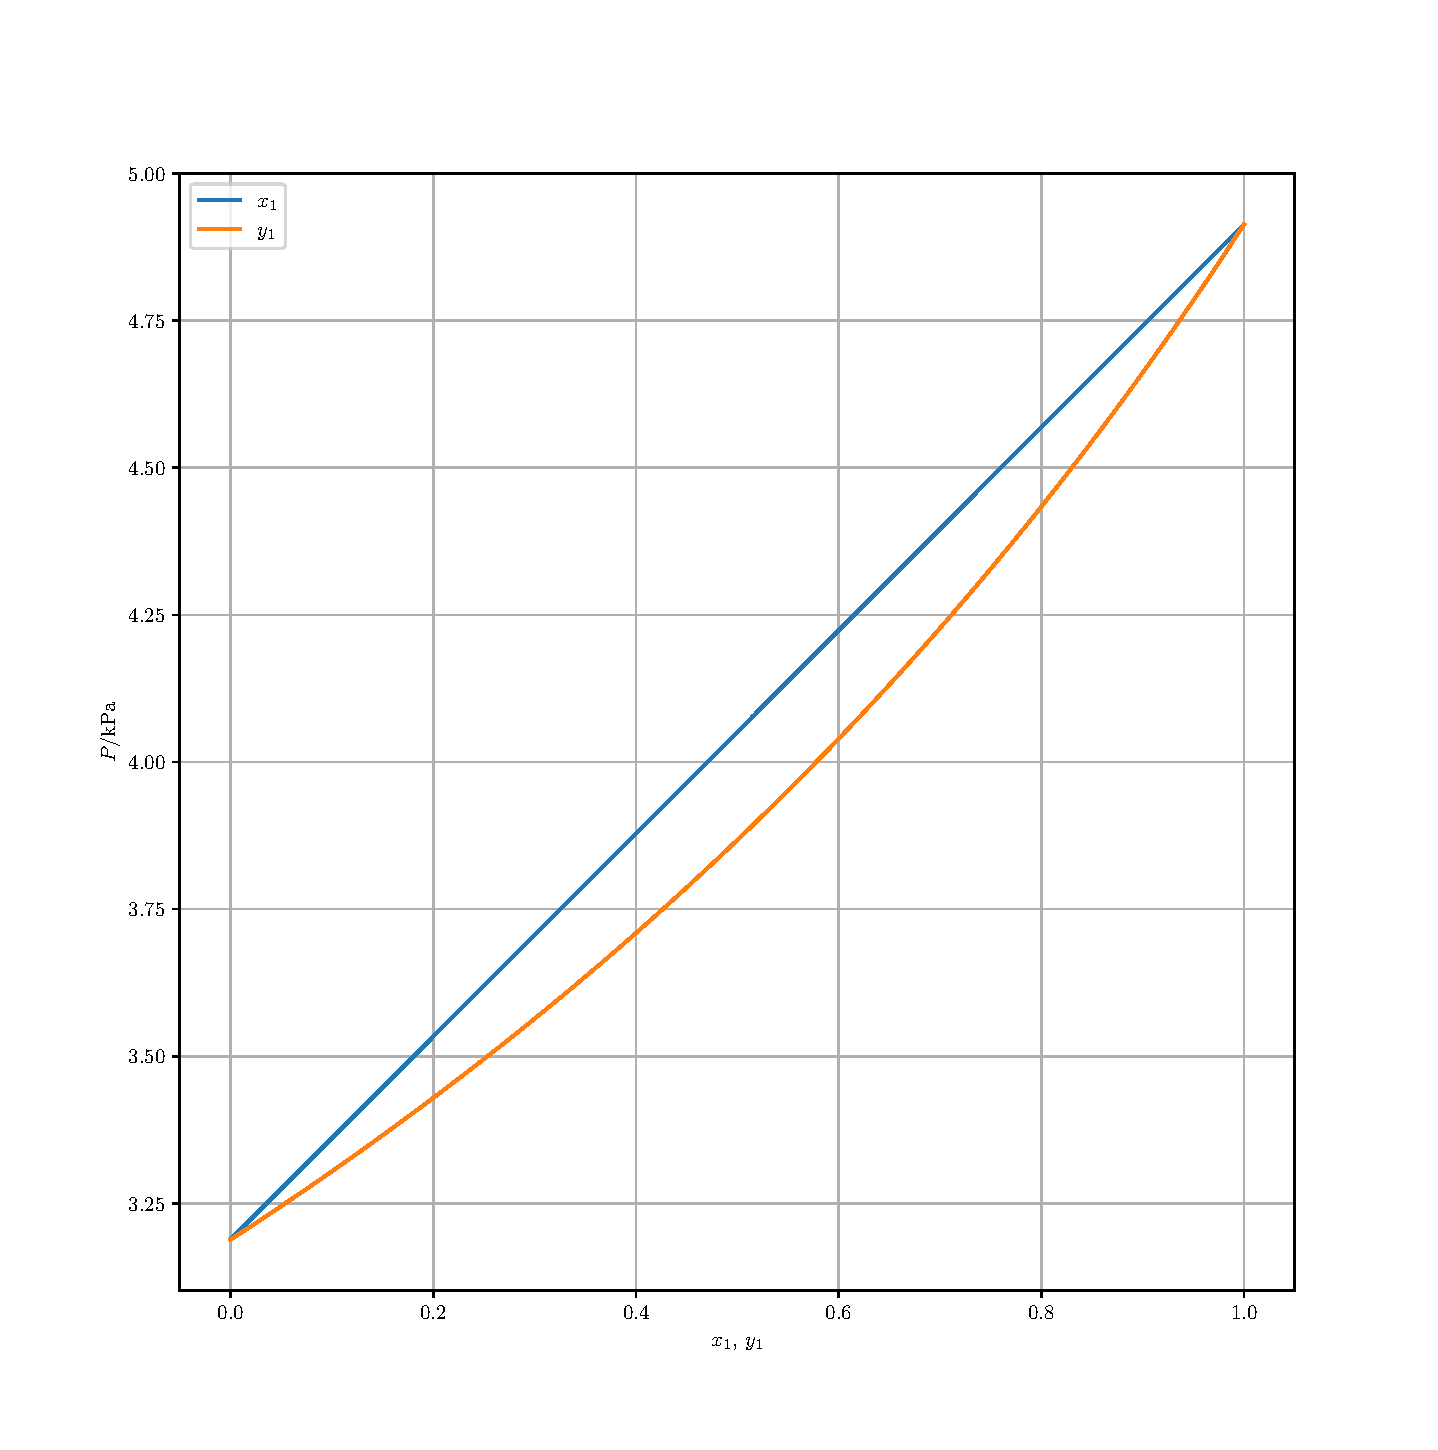
\includegraphics[scale=0.3]{images/problem_10_2a.pdf}
      \caption{$P-x-y$ diagram of the system described in Problem 10.2.}
      \label{fig:p10_2}
    \end{minipage}
    \hfill
    insert other figure here
    \begin{minipage}[t]{0.45\textwidth}
    \end{minipage}
  \end{figure}
\end{solution}

\subsection*{Problem 10.3}
\addcontentsline{toc}{subsection}{Problem 10.3}

\subsection*{Problem 10.9}
\addcontentsline{toc}{subsection}{Problem 10.9}
A mixture containing equimolar amounts of benzene(1), toluene(2), and
ethylbenzene(3) is flashed to conditions $T$ and $P$. For one of the
conditions following determine the equilibrium mole fractions
{$x_{i}$} and $\{y_{i}\}$ of the liquid and vapor phases formed and
the molar fraction $\mathcal{V}$ of the vapor formed. Assume that
Raoult's law applies.
\begin{enumerate}[label=(\alph*)]
  \item $T=110~\unit{\degreeCelsius}$, $P=90~\unit{\kilo\pascal}$
  \item $T=110~\unit{\degreeCelsius}$, $P=100~\unit{\kilo\pascal}$
  \item $T=110~\unit{\degreeCelsius}$, $P=110~\unit{\kilo\pascal}$
  \item $T=110~\unit{\degreeCelsius}$, $P=120~\unit{\kilo\pascal}$
\end{enumerate}
\begin{solution}
  \begin{gather*}
    P_{i}^{\text{sat}} = \exp \left(A_{i} - \frac{B_{i}}{T + C_{i}}\right) \\
  \end{gather*}
  \begin{gather*}
    k_{i} = \frac{P_{i}^{\text{sat}}}{P} \\
  \end{gather*}
  \begin{gather*}
    1 = \sum_{i}\frac{z_{i}k_{i}}{1 + \mathcal{V}(k_{i} - 1)}
  \end{gather*}
  \begin{gather*}
    y_{i} = \frac{z_{i}k_{i}}{1 + \mathcal{V}(k_{i} - 1)} \\
    x_{i} = \frac{y_{i}P_{i}^{\text{sat}}}{P}
  \end{gather*}
  \begin{empheq}[box=\widefbox]{align*}
    \mathcal{V} =
    0.834,
    0.573,
    0.349,
    0.143,
  \end{empheq}
  \begin{empheq}[box=\widefbox]{align*}
    x =
    \begin{bmatrix}
      0.143 \\ 0.306 \\ 0.551
    \end{bmatrix},
    \begin{bmatrix}
      0.188 \\ 0.334 \\ 0.477
    \end{bmatrix},
    \begin{bmatrix}
      0.239 \\ 0.345 \\ 0.416
    \end{bmatrix},
    \begin{bmatrix}
      0.293 \\ 0.342 \\ 0.365
    \end{bmatrix}
  \end{empheq}
  \begin{empheq}[box=\widefbox]{gather*}
    y =
    \begin{bmatrix}
      0.371 \\ 0.339 \\ 0.290
    \end{bmatrix},
    \begin{bmatrix}
      0.441 \\ 0.333 \\ 0.226
    \end{bmatrix},
    \begin{bmatrix}
      0.509 \\ 0.312 \\ 0.179
    \end{bmatrix},
    \begin{bmatrix}
      0.573 \\ 0.342 \\ 0.144
    \end{bmatrix}
  \end{empheq}
\end{solution}

\subsection*{Problem 10.17}
\addcontentsline{toc}{subsection}{Problem 10.17}
For the system ethyl ethanoate(1)/\textit{n}-heptane(2) at
$343.15~\unit{\kelvin}$.
\begin{align*}
  \ln \gamma_{1} = 0.95 x_{2}^{2} & \ln \gamma_{2} = 0.95 x_{1}^{2} \\
  P_{1}^{\text{sat}} = 79.80~\unit{\kilo\pascal} & P_{2}^{\text{sat}}
  = 40.50~\unit{\kilo\pascal}
\end{align*}
Assuming the validity of Eq.~\ref{eq:MRL}
\begin{equation}
  y_{i}P = \gamma_{i}x_{i}P_{i}^{\text{sat}}
  \label{eq:MRL}
\end{equation}
\begin{enumerate}[label=(\alph*)]
  \item Make a BUBL P calculation for $T=343.15~\unit{\kelvin}$, $x_{1}=0.05$.
  \item Make a DEW P calculation for $T=343.15~\unit{\kelvin}$, $y_{1}=0.05$.
  \item What is the azeotrope composition and pressure at
    $T=343.15~\unit{\kelvin}$?
\end{enumerate}
\begin{solution}
  \begin{enumerate}[label=(\alph*)]
    \item
      \begin{gather*}
        P = x_{1}\gamma_{1}P_{1}^{\text{sat}} +
        x_{2}\gamma_{2}P_{2}^{\text{sat}}
      \end{gather*}
      \begin{empheq}[box=\widefbox]{gather*}
        P = 47.971~\unit{\kilo\pascal} \\
        y_{1} = 0.196
      \end{empheq}
  \end{enumerate}
\end{solution}

\end{document}
